\documentclass[12pt,a4paper]{article}
\usepackage[margin=2.5cm,left=2cm,includefoot]{geometry}
\usepackage{hyperref}
\usepackage{array}
\usepackage{enumitem}
\usepackage{graphicx}
\usepackage[section]{placeins}
\usepackage{titlesec}

\setlength{\parindent}{0em}

\graphicspath{{Images/}}

% Header and footer
\usepackage{fancyhdr}
\pagestyle{fancy}

\rhead{COS 301}
\lhead{Team Objective C}
\fancyfoot{}
\fancyfoot[R]{Page \thepage}

\renewcommand{\headrulewidth}{2pt}
\renewcommand{\footrulewidth}{1pt}

\begin{document}

\begin{titlepage}
  \begin{center}
    \begin{figure}[t]
      \centering
      
\includegraphics[width=350px]{logo.PNG}
     \end{figure}
     
     \textsc{\LARGE COS301 Group Task 2 \newline \newline Architectural Design\\[0.5cm] Specifications}
     
     \textbf{\newline Team Objective C} \\
     \begin{flushright} \large
      Diana Obo \emph{u13134885}\newline
      Kamogelo Tsipa \emph{u13010931}\newline
      Linda Zwane \emph{u14199468}\newline
      Melvin Zitha \emph{u12138747}\newline
      Minal Pramlall \emph{u13288157}\newline
      Rotondwa Siavhe \emph{u????????}\newline
       \end{flushright} 
      \vfill %whitespace
      
      Team Objective C Github: \href{https://github.com/ShockwaveZA/Objective-C-Team}{Github} page.\\
      \url{https://github.com/ShockwaveZA/Objective-C-Team}
      
      \vfill
      {\large Date:}
      \\
      {\large \today}
     \end{center}
    \end{titlepage}


\tableofcontents
\newpage

\section{Design Constraints}
	\begin{itemize}
		\item The NavUp application must at least have basic navigation system functionalities.
		\item The location  of the user must be determined both indoors and outdoors.
		\item The NavUp system will be integrated into the Computer Science department's website.
		\item The NavUp system should allow the integration of a variety of services were navigation is the main objective.
		\item The NavUp application must only allow the administrator to create, update and delete information about events, venues and activities.
		\item The user’s password should be stored in the database in encrypted format.
		\item A signed up user can only request services from the various modules.
		\item A user can change any field value except the isAdmin field.
		\item The administrator is the only one that can change the isAdmin filed value of other users.
 
		
	\end{itemize}
    
\section{External Interface Requirements}
This section will cover the requirements of the external interface of the NavUP system. NavUP is going to be designed to operate as a mobile applications for smart devices such as smart phones and tablets; as such, the minimum requirements will fall in line with a typical entry-level smart device that is capable of running mobile applications.\newline

    \subsection{Minimum Requirements}
        \begin{itemize}
            \item 768x1024 minimum resolution
            \item Android, Apple or Windows Mobile Operating Systems
            \item WiFi enabled
            \item Internet coverage
        \end{itemize}
     
        \subsection{User interface}
        When the user is navigating they must be able to see a search box where they can enter a location they want to travel to. Their current location should be visible on the map, see fig1: Navigation.The points of interest will be shown in a list of different categories, when you click on a category it will show you a more specific list of what you want; eg. clicking on ATMs will show a list consisting of FNB, ABSA, Capitec and Nedbank,see fig2: Points of Interest. For the events module you will be given two options, either view all events or request to add an event, see fig3 events. The Fitness module should allow the user to add their daily, weekly or monthly goals. It will show the statistics of the day and green button if they have achieved their goal or else a red button if they have not, see fig4 Fitness.
        \begin{figure}
                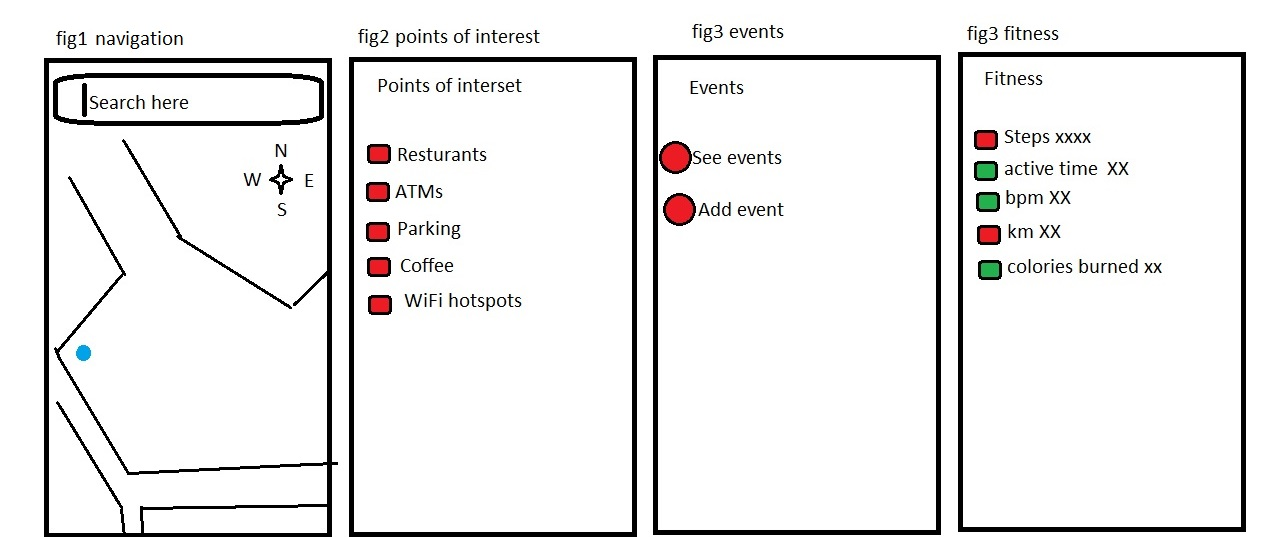
\includegraphics[width=\linewidth]{Images/userInterface.jpg}
                \caption{User Interface Design}
        \end{figure}
        
        \subsection{Hardware interface}
        The NavUP system will be greatly dependent upon the user's device hardware system. Which must be a mobile device such as a laptop, smartphone, tablet or tablet.

        \subsection{Software interface}
        The NavUP system will be greatly dependent upon the user's device operating system which could be either Android OS, Windows OS or Apple iOS. The database will be a vital part of the system because it will get information from the user and send it to Google Maps, then return the result of the search query back to the user. The database will also be responsible for storing data about places of interest the user might be interested in. It will store the data regarding to when and where events are taking place and distance walked for the fitness module. 

        \subsection{Communications interface}
        All of the types of users will be making use of the HTTP protocol to communicate with the program interfaces and as well as FTP for media upload if they want to transfer their profile picture or a picture for an event if they have admin priviledges.

\section{Technology choices}
        \subsection{Android SDK}
        The Android SDK has useful developent tools which will be needed for the NavUP system. Android allows applications access to the location services compatible with the device. The LocationManager system service provides APIs to determine location and bearing of the device.
        \subsection{WiFi}
        WiFi is widely available on campus for both students and guests.It will be used to allow users/guest to connect to the internet so they can make use of the the NavUP system.
        \subsection{Database Server}
        The database will be responsible for the storage of data, since the information that is required to be stored is structured, SQL is the most logical choice.
     	
\section{UML}
	\subsection{UML - User}
	The architecture of the User group is decidedly much simpler than the other modules as the user module is characterized mainly by the Template Design Pattern.
	\begin{figure}
		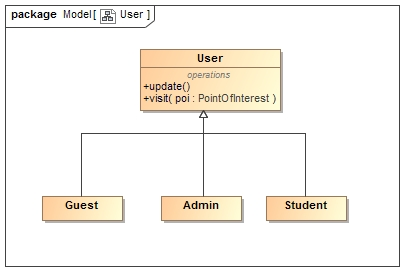
\includegraphics[width=\linewidth]{Images/User.jpg}
		\caption{Class diagram of the User objects}
	\end{figure}
	
	\subsection{UML - Events}
	The modelling of the Events module will be characterized by the Observer design pattern, since the EventHandler will attach the users that are willing to participate, and will use the notify() method to communicate with only the participants of the event not a user that does not want to participate and just happens to be in proximity of event.
	\begin{figure}
		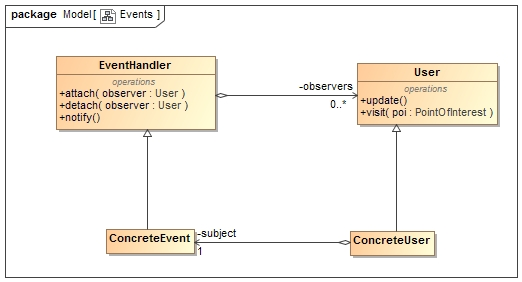
\includegraphics[width=\linewidth]{Images/Events.jpg}
		\caption{Class diagram of the Events module}
	\end{figure}
	
	\begin{figure}
		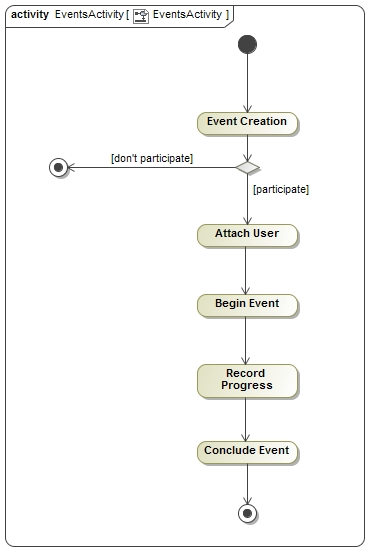
\includegraphics[width=\linewidth]{Images/EventsActivity.jpg}
		\caption{Activity diagram of the Events module}
	\end{figure}
	
	\subsection{UML - Fitness}
	The Fitness module, like Events, will also be using the Observer Design Pattern. The FitnessObserver will be used by Navigation to monitor the user and simply track the activity, rewarding the user by achieving milestones.
	\begin{figure}
		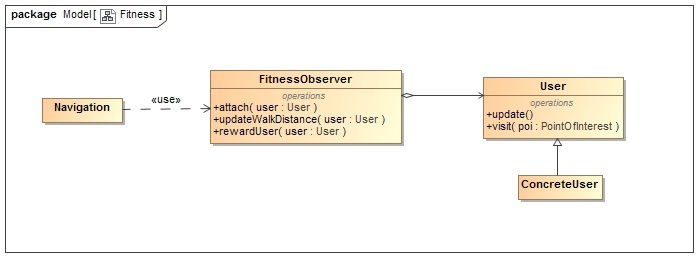
\includegraphics[width=\linewidth]{Images/Fitness.jpg}
		\caption{Class diagram of the Fitness module}
	\end{figure}
	
	\begin{figure}
		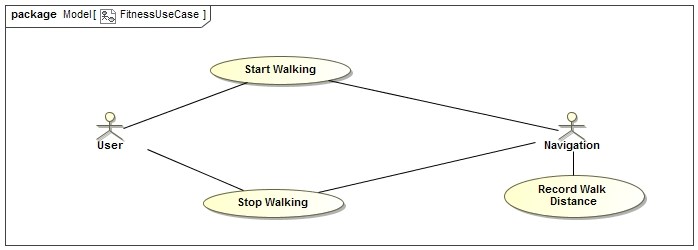
\includegraphics[width=\linewidth]{Images/FitnessUseCase.jpg}
		\caption{Use Case diagram of the Fitness module}
	\end{figure}
	
	\subsection{UML - Navigation}
	The Navigation module will make use of the Memento Design Pattern, the needs of this module is to save routes as well as perform remove and update operations. Memento best suits this need because of the Caretaker class that stores instances, or an entire route in this particular case.
	\begin{figure}
		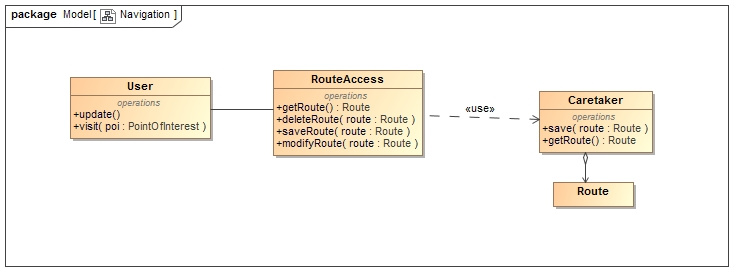
\includegraphics[width=\linewidth]{Images/Navigation.jpg}
		\caption{Class diagram of the Navigation module}
	\end{figure}
	
	\begin{figure}
		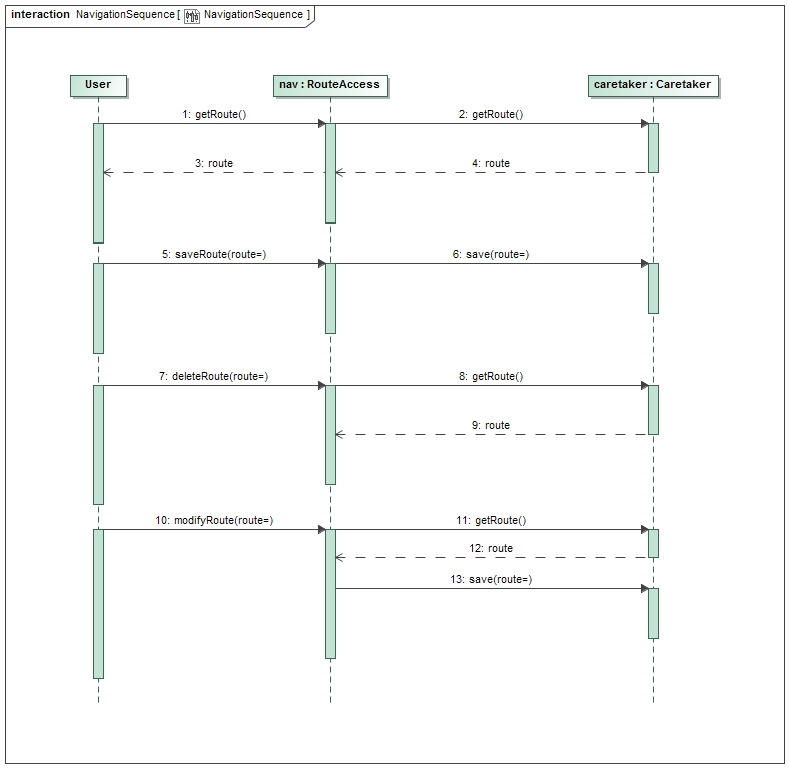
\includegraphics[width=\linewidth]{Images/NavigationSequence.jpg}
		\caption{Sequence diagram of the Navigation module}
	\end{figure}
	
	\subsection{UML - Points of Interest}
	The Points of Interest module will be using the Visitor Design Pattern, when a user is walking around and visits a point of interest, an event will be triggered. This event will provide the user with information of this point of interest and may also record that the user has visited this location in this instance (This may help with Surveillance).
	\begin{figure}
		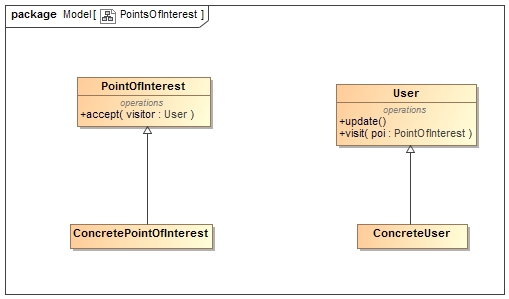
\includegraphics[width=\linewidth]{Images/PointsOfInterest.jpg}
		\caption{Class diagram of the Points of Interest module}
	\end{figure}
	
	\begin{figure}
		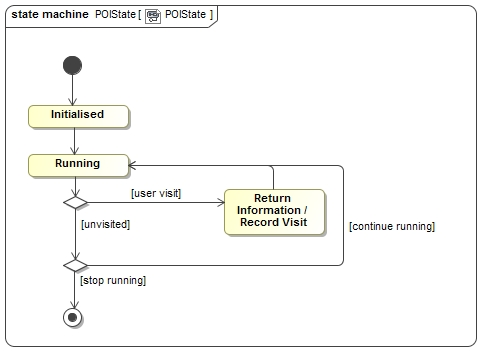
\includegraphics[width=\linewidth]{Images/POIState.jpg}
		\caption{State diagram of the Points of Interest module}
	\end{figure}
	
\section{Quality and feasibility of design}
Given the scope of the NavUP system, we must ensure that the operational requirements of the system, and their incorporation into design requirements, can be converted into a finished product. Given the design constrains, see Design constraints, the NavUP system will reliably provide users with basic operational requirements such as navigation functionalities and access to a wealth of information on campus about events, venues and points of interests based on user input. The design checks and validates input from the user to ensure that the results returned are correct and complete, in a consistent manner. In cases where the user has entered anything incorrectly, the robust design of the system will enable it to still behave as expected or stop and request the user to enter the details again. \newline

When it comes to efficiency, the NavUP system operates on any device that matches the minimum requirements, see minimum requirements. WIFI, cellular or Global positioning system (GPS) network will be used to communicate efficiently with the server. The system will also be able to perform under abnormal conditions, such as when the WIFI network is not available, cellular network will be used to allow the user to use the application. \newline

To make sure that maintainability of the system is easy, it is divided into different modules. The modules contain within them, subsystems which allow for additional features to be added or removed. The systems modular design allows it to continue operating if other modules fail to respond. \newline

The general usability of the application allows users of all levels the ability to use the application. As with the user interface, see External Interface Requirements, it is designed to allow users access to basic features of the application. User input validation will be used to make sure that users enter the correct information and the correct information is sent back to the user. \newline	

\end{document}
